
Quench velocity before quench detection has been estimated numerically. The magnetic field inside the magnet varies in the range of $B \in (0, 3)~\text{T}$. Therefore, 7 separate 1D analysis have been conducted in ANSYS to estimate quench velocity as a function of time and magnetic field.

\begin{figure}[ht!]
    \centering
    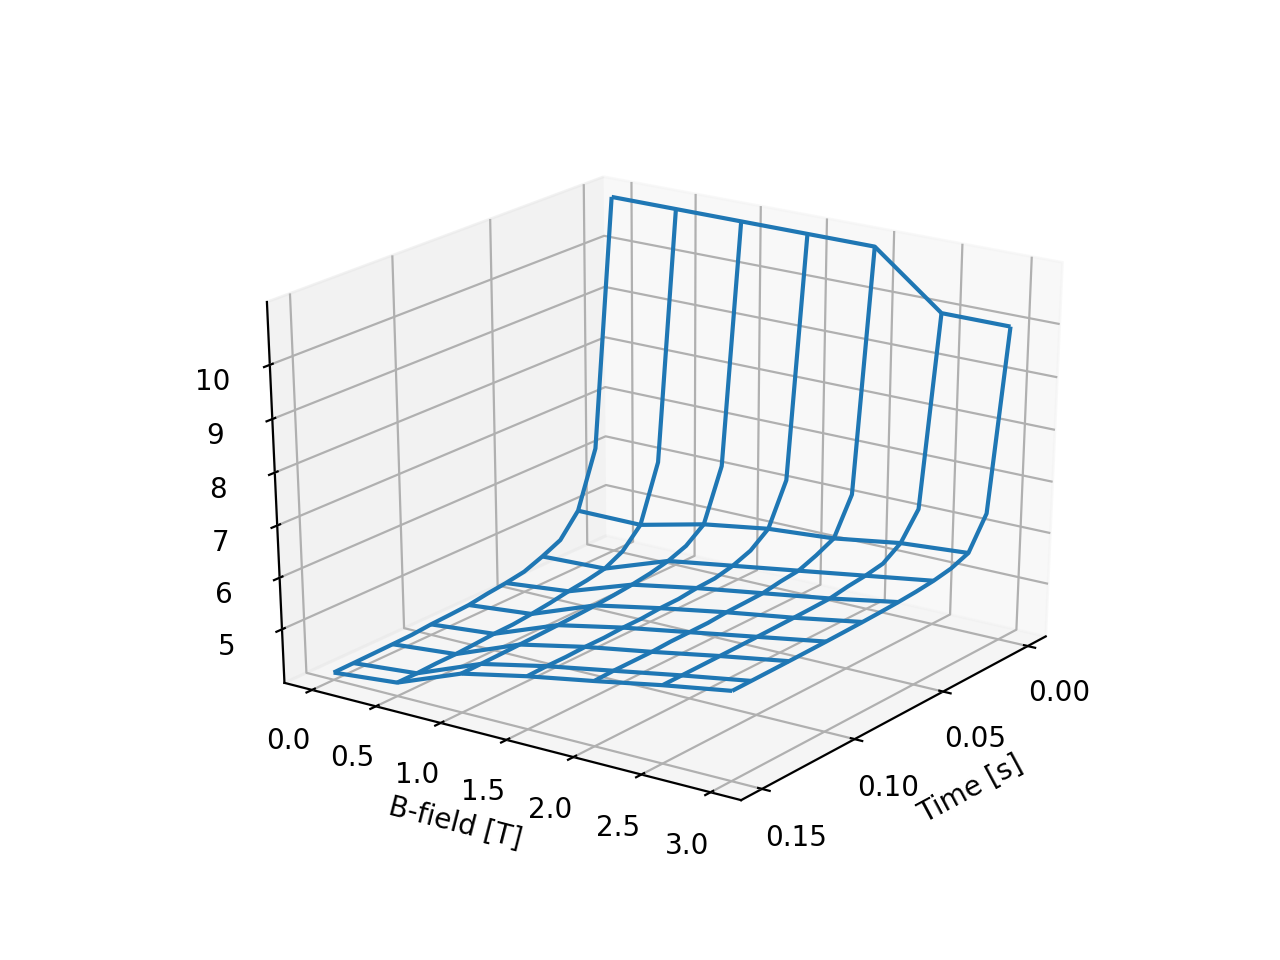
\includegraphics[width=0.6\linewidth]{figures/skew_quad_bcs/magnetic_field_mapping/Quench_Velocity_Map.png}
    \caption{Quench Velocity as a function of time and magnetic field strength}
    \label{fig:Q_v_map}
\end{figure}

\begin{figure}[H]
\centering
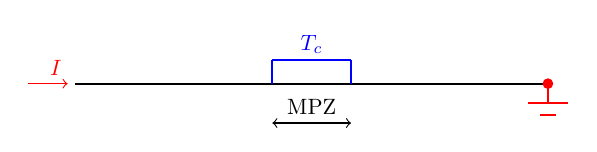
\begin{tikzpicture}[scale = 1]
\draw[thick, black] (-3,0) -- (3,0);
\filldraw[red] (3,0) circle (0.06);
\draw[thick, red] (3,0) -- (3,-0.25);
\draw[thick, red] (2.75,-0.25) -- (3.25,-0.25);
\draw[thick, red] (2.9,-0.4) -- (3.1,-0.4);
\draw[thin, red, ->] (-3.6,0) -- (-3.1,0);
\draw[thick, blue] (-0.5,0) -- (-0.5,0.3);
\draw[thick, blue] (-0.5,0.3) -- (0.5,0.3);
\draw[thick, blue] (0.5,0.3) -- (0.5,0);
\draw[thin, black, <->] (-0.5,-0.5) -- (0.5,-0.5);
\node[scale=0.8] at (0,-0.3) {MPZ};
\node[scale=0.8, blue] at (0,0.5) {$T_\text{c}$};
\node[scale=0.8, red] at (-3.25,0.2) {$I$};
\end{tikzpicture}
\caption{Simulation settings}
\label{fig:sim_settings_1}
\end{figure}

% \begin{figure}[H]
% \centering
% \begin{tikzpicture}[scale = 1]
% \draw[thick, black] (-3,0) -- (3,0);
% \filldraw[red] (3,0) circle (0.06);
% \draw[thick, red] (3,0) -- (3,-0.25);
% \draw[thick, red] (2.75,-0.25) -- (3.25,-0.25);
% \draw[thick, red] (2.9,-0.4) -- (3.1,-0.4);
% \draw[thin, red, ->] (-3.6,0) -- (-3.1,0);
% \draw [thick, red] (-0.5,0) .. controls +(0:0.6cm) and +(180:0.3cm) .. (0,0.6);
% \draw [thick, red] (0,0.6) .. controls +(0:0.3cm) and +(180:0.6cm) .. (0.5,0);
% \draw[thin, black, <->] (-0.5,-0.5) -- (0.5,-0.5);
% \node[scale=0.8] at (0,-0.3) {2 mm};
% \node[scale=0.8, red] at (0,0.8) {$T_\text{peak}$};
% \node[scale=0.8, red] at (-3.25,0.2) {$I$};
% \end{tikzpicture}
% \caption{Simulation settings}
% \label{fig:sim_settings_2}
% \end{figure}

\begin{figure}[H]
\centering
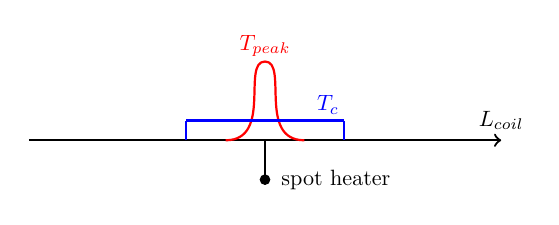
\begin{tikzpicture}[scale = 1]
\draw[thick, black, ->] (-3,0) -- (3,0);
\filldraw[black] (0,-0.5) circle (0.06);
\draw[thick, black] (0,0) -- (0,-0.5);
\draw [thick, red] (-0.5,0) .. controls +(0:0.6cm) and +(180:0.3cm) .. (0,1);
\draw [thick, red] (0,1) .. controls +(0:0.3cm) and +(180:0.6cm) .. (0.5,0);
\draw[thick, blue] (-1,0) -- (-1,0.25);
\draw[thick, blue] (-1,0.25) -- (1,0.25);
\draw[thick, blue] (1,0.25) -- (1,0);
\node[scale=0.8, black] at (0.9,-0.5) {spot heater};
\node[scale=0.8, black] at (3,0.25) {$L_\text{coil}$};
\node[scale=0.8, blue] at (0.8,0.45) {$T_\text{c}$};
\node[scale=0.8, red] at (0,1.2) {$T_\text{peak}$};
\end{tikzpicture}
\end{figure}

\begin{figure}[H]
\centering
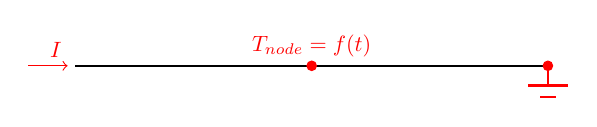
\begin{tikzpicture}[scale = 1]
\draw[thick, black] (-3,0) -- (3,0);
\filldraw[red] (3,0) circle (0.06);
\draw[thick, red] (3,0) -- (3,-0.25);
\draw[thick, red] (2.75,-0.25) -- (3.25,-0.25);
\filldraw[red] (0,0) circle (0.06);
\draw[thick, red] (2.9,-0.4) -- (3.1,-0.4);
\draw[thin, red, ->] (-3.6,0) -- (-3.1,0);
\node[scale=0.8, red] at (0,0.25) {$T_\text{node}= f(t)$};
\node[scale=0.8, red] at (-3.25,0.2) {$I$};
\end{tikzpicture}
\caption{Simulation settings}
\label{fig:sim_settings_3}
\end{figure}


% Analysis assumptions:
% No helium cooling
% Power input heats up the coil directly (no intermediate insulation layer) 
% Temperature in the windings’ cross-sectional area is uniform - 1D element
% Longitudinal heat transfer inside the insulation is negligible with respect to windings - 1D element


% Winding: 	link68, thermo-electric 1D elements for heat conduction + Joule heating
% Insulation: 	link33, thermal 1D elements for heat conduction



% Resistive voltage curve changes the slope during the analysis, - turn-to-turn propagation occurs in the model

% Turn-to-turn propagation occurs to slow compared to measurements-assumptions related to insulation elements are too conservative

% In measurements, quench spot is applied through insulation  direct power input in simulations ought to be modified

% Exact value of RRR of the measured magnet needs to be verified with INFN 


% Preparation of thermo-magneto-electric model to simulate current discharge

% Preparation of magnetic model in ANSYS to simulate magnetic field change during discharge (influence of iron yoke)
% Coupling of ANSYS quench velocity model with circuit in PSpice 
% Validation against measurements from INFN


\begin{figure}
\centering
\begin{tikzpicture}
\pgfplotsset{
    scale only axis,
    height=4cm,
    width=8cm,
    compat=1.3,
    scaled x ticks=base 10:0,
    xmin=0, xmax=9
}
\begin{axis}[
  axis y line*=left,
  ymin=0, ymax=20,
  xlabel={Time, s},
  ylabel={Resistive Voltage, V},
]
\addplot[smooth, red] table[x=Time,y=Resistive_Voltage,col sep=comma] {figures/skew_quad_bcs/current_voltage_discharge.csv}; 
\label{plot_resistive_voltage}
\end{axis}

\begin{axis}[
  axis y line*=right,
  axis x line=none,
  ymin=0, ymax=100,
  ylabel={Current, A}
]
\addplot[smooth, blue] table[x=Time,y=Current,col sep=comma] {figures/skew_quad_bcs/current_voltage_discharge.csv}; 
\label{current}
\addlegendentry{$I$}
\addlegendimage{/pgfplots/refstyle=plot_resistive_voltage}\addlegendentry{$V_\text{r}$}
\end{axis}
\end{tikzpicture}
\caption{Current and Resistive Voltage change during the discharge of skew quadrupole}
\label{fig:skew_quad_discharge}
\end{figure}


\begin{figure}
\centering
\begin{tikzpicture}
\pgfplotsset{
    scale only axis,
    height=4cm,
    width=8cm,
    compat=1.3,
    scaled x ticks=base 10:3,
    xmin=0, xmax=0.15
}
\begin{axis}[
  axis y line*=left,
  ymin=0, ymax=0.35,
  xlabel={Time, s},
  ylabel={Resistive Voltage, V},
]
\addplot[smooth, red] table[x=Time,y=Resistive_Voltage,col sep=comma] {figures/skew_quad_bcs/current_voltage_quench_detection.csv}; 
\label{plot_resistive_voltage}
\end{axis}

\begin{axis}[
  axis y line*=right,
  axis x line=none,
  ymin=0, ymax=100,
  ylabel={Current, A},
  legend pos=south east
]
\addplot[smooth, blue] table[x=Time,y=Current,col sep=comma] {figures/skew_quad_bcs/current_voltage_quench_detection.csv}; 
\label{current}
\addlegendentry{$I$}
\addlegendimage{/pgfplots/refstyle=plot_resistive_voltage}\addlegendentry{$V_\text{r}$}
\end{axis}
\end{tikzpicture}
\caption{Current and Resistive Voltage change during the discharge of skew quadrupole}
\label{fig:skew_quad_discharge}
\end{figure}